\documentclass[]{usiinfprospectus}

\usepackage[utf8]{inputenc}
\usepackage[english]{babel}
\usepackage[T1]{fontenc}

\captionsetup{labelfont={bf}}

\author{Carlos Eduardo B. Bezerra}

\title{A fault tolerant multi-server system for MMOGs}
%\subtitle{A crash-stop model oriented approach}
\versiondate{\today}
  
\begin{committee}
%With more than 1 advisor an error is raised...: only 1 advisor is allowed!
\researchadvisor[Universit\`a della Svizzera Italiana, Switzerland]{Prof.}{Fernando}{Pedone}
\academicadvisor[Universit\`a della Svizzera Italiana, Switzerland]{Prof.}{Fernando}{Pedone}
\committeemember[Universit\`a della Svizzera Italiana, Switzerland]{Prof.}{Committee}{Member1}
\committeemember[Universit\`a della Svizzera Italiana, Switzerland]{Prof.}{Committee}{Member2}
%\committeemember[Universit\`a della Svizzera Italiana, Switzerland]{Prof.}{Committee}{Member3}
\coadvisor[Universidade Federal do Rio Grande do Sul, Brazil]{Prof.}{Cl\'audio}{Geyer}
%\coadvisor[Universit\`a della Svizzera Italiana, Switzerland]{Prof.}{Research}{Co-Advisor2}
%\coadvisor[Universit\`a della Svizzera Italiana, Switzerland]{Prof.}{Research}{Co-Advisor3}
\phddirector{Prof.}{Michele}{Lanza}
\end{committee}

\abstract {
MMOGs -- massively multiplayer online games -- have become, in the last decade, an important genre of online entertainment, having a significant market share. In these games, many thousands of participants play simultaneously with one another in the same match. However, this kind of game is traditionally supported by a powerful (and expensive) central infrastructure with considerable cpu power and very fast and low latency Internet connections. This work proposes the use of a geographically distributed server system, formed by voluntary nodes which help serving the game to the players. Two very important features, therefore, must be provided: consistency (which may be week and only existing in the players' perspective) and fault tolerance, as some of the participating nodes may crash and become unavailable. For this work, we consider the crash-stop failure model.
}
 

\begin{document}
\maketitle

%%%%%%%%%%%%%%%%%%%%%%%%%
\section{Introduction} \label{sec:introduction}
%%%%%%%%%%%%%%%%%%%%%%%%%

MMOGs emerged in the last decade as a new trend because of the decrease of the domestic Internet connection cost and the increase of its average bandwidth. This kind of games have become very popular because they allow the online interaction of a massive number of players at the same time. In the most succesful cases, such as World of Warcraft \cite{worldofwarcraft}, Lineage II \cite{lineage2} and EVE Online \cite{eveonline}, for example, tens of thousands of players are supported simultaneously \cite{chen2006pch}. In these games, the players can interact with one another in a virtual environment.

Generally, each player controls an entity called \emph{avatar}, which is his representation in the virtual environment -- a character who executes the orders given by the player, therefore interfering in the outcome of the game. To provide a consistent view among the different participants, every action performed by each avatar is processed by a server, which calculates the game state resulting from such action. This new state is then broadcast to the players to whom it might be relevant -- again, the state itself does not need to be consistent, but only what the players see.

To cope with the receiving and processing of thousands of actions and the broadcast of their respective resulting states, the traditional approach is to use a large central server -- usually a cluster with a high-speed, low latency Internet connection -- which provides such cpu power and network capabilities \cite{feng2007wnn}. Decentralized alternatives could be used, so that such expensive infrastructure would not be necessary. For example, a fully decentralized system could be used, where each player is a peer responsible for calculating a portion of the game state and for synchronizing it with other peers \cite{rieche2007ppb, hampel2006ppa, elrhalibi2005abm, iimura2004zfg, knutsson2004pps}.

In such peer-to-peer approach, the players would need to agree upon the outcome of the actions, in order for their view to be consistent. To reduce the traffic between peers, the state updates could be sent only to whom they are relevant. To define what is relevant for each player, the virtual environment could be divided into regions \cite{schiele2007rpp}, so that a small peer group would be formed by players who were inside each of these regions. Players whose avatars were in a given region could form a smaller peer-to-peer group -- possibly reducing also the cost of each agreement -- and their own computers would decide the outcome of the players' actions in that area of the virtual environment. Unfortunately, however, the fully decentralized approach would imply a heavy communication cost on the players, specially when running some agreement protocol. This might not only degrade the quality of the game, but also increase the requirements imposed on the players' computational resources, therefore likely reducing their number.

We propose here, then, a system composed of geographically distributed nodes which may act as game servers -- these nodes could be provided, for example, by volunteers or by companies which might have some commercial interest with the game being hosted. Some works, such as \cite{assiotis2006dam,ng2002msa, chertov2006olb, lee2003sdl} also propose the use of a distributed server, but they consider that the nodes are connected through a high speed and low latency network (e.g. a cluster), what makes their solutions only partially applicable in a scenario with highly dynamic and volatile resources, such as wide-area networks formed with volunteer resources. Such networks have some inherent problems: nodes with low availability and dependability, low bandwidth and low processing power compared to current dedicated MMOG servers maintained by large game companies.

The rest of this document is organized as follows: Section \ref{sec:model} gives an overview of the system model and describes briefly some of its protocols; Section \ref{sec:futurework} presents the research directions to be followed next and Section \ref{sec:achievements} lists some of the accomplishments achieved by this research so far.

%%%%%%%%%%%%%%%%%%%%%%%%%
\section{Proposed model} \label{sec:model}
%%%%%%%%%%%%%%%%%%%%%%%%%


We consider here persistent state real-time games with virtual environments where each player controls an avatar by issuing commands to it. Through the avatar, the player interacts with the virtual world and with objects present in it, such as avatars from other players. The basic operation of the game network support system must be as follows: when a player connects to the server, it must send the current state of the player's avatar and of the surroundings of its current location; after that, this player keeps receiving periodic state updates for the objects which are relevant to it (usually based on whether those objects may be seen by the player \cite{bezerra2008a3,ahmed2008dai,minson2005aim}). When a player issues a command (e.g. move his avatar from one place to another, pick up an object, attack another player's avatar etc.), it is sent as a message to the server, which processes it and decides its outcome, probably changing the state of the game, which is then broadcast to all involved players.

The next sections will describe the services the service must provide to the players connected to it (Section \ref{sec:services}), the specific requirements for a fault-tolerant distributed MMOG server system, considering the crash-stop failure model, as well as the proposed distributed architecture (Section \ref{sec:distserver}) and an algorithm devised to synchronize the game state between the replicas (Section \ref{sec:algorithm}).

\subsection{Services to be provided} \label{sec:services}

As already mentioned, in order to provide the services required by the MMOG, this work proposes the use of a geographically distributed system composed of voluntary nodes working together to form a distributed MMOG server. This distributed server must deliver, at least, the following services:

\begin{itemize}
	\item \textbf{Simulation} of the game, that is, the receiving of actions sent by the players and then processing their corresponding outcomes, which may result in changes to the game state;
	\item \textbf{Broadcasting} a portion of the current game state to the different players connected to it;
	\item \textbf{Storage} of the game state, that is, the combination of the states of each object in the virtual environment.
\end{itemize}

It is important to note that in real-time games (as opposed to turn-based games), due to the possibly fast-paced interaction of the players, it is critical to provide \textbf{timeliness} for the delivery of state update messages to them, so that they have the illusion of a common environment. Besides, it is necessary to provide \textbf{consistency} for the game state between each pair of players interacting with one another, which means that the game state they perceive must be as similar as possible. Although it is very hard to guarantee that every player will share the exact same view, it is important for their commands to be processed as if there was a single, strongly consistent game state, which is the one stored at the server. 


%%%%%%%%%%%%%%%%%%%%%%%%%
\subsection{Distributed server system} \label{sec:distserver}

The main purpose of the system is to reduce or, ideally, eliminate the necessity of a central server for the game. In this work, the approach proposed to achieve this is based on principles similar to those of volunteer computing, where a potentially large set of contributors make their computers available to perform tasks requested by some remote entity. With such a system, although each of these nodes is probably much less powerful than a traditional mmog server, when working together they can sum up the cpu power and network link necessary to host one of these games.

However, several questions arise when dealing with a potentially large scale geographically distributed server system composed of voluntary nodes. First, as the nodes are volunteer, there is no guarantee that they will be available whenever they are needed, neither there is any guarantee regarding the amount of resources that each of these nodes makes available for the system -- be it cpu power, network bandwidth or storage capability. Group communication may also be a problem, since primitives for that -- such as network level multicast -- are not widely available on the Internet.

Finally, considering the potentially large number of nodes in this system, it is very likely that some of them present failures, for what we are assuming the crash-stop failure model -- therefore, we assume the possibility of nodes crashing and network links becoming unavailable. The services provided by the system must continue even in the presence of such failures. Not only must the distribution itself be transparent to the players, but also the existence of failures and their countermeasures must not be noticeable by them.

In Section \ref{sec:statepart}, we describe how the game state will be distributed among the different server nodes; in Section \ref{sec:consprot}, a preliminary consistency management protocol, based on state machine replication, is presented.

%%%%%%%%%%%%%%%%%%%%%%%%%
\subsubsection{State partitioning} \label{sec:statepart}

In order to split a game server into several smaller units executed by many volunteer nodes, it is used the idea of dividing the virtual environment in regions, each of which being managed by a different server. There are many approaches proposed in the literature, such as using fixed size cells which are grouped into regions, or using binary space partition trees, and so on. For the sake of generality, the architecture proposed here  does not decide how exactly the partitioning of the virtual environment will be performed. To cope with the possibility of failures, each server has several replicas, forming a server group.

The state partitioning is performed based on what objects are located in each region. The state of a object is managed, then, by the server group assigned to the region where that object is located. This way, the locality of data is explored: objects closed to each other are more likely to interact and, as they are located on the same server group, their interaction should be faster. Besides, by exploring the locality of the game data (state of the objects), the inter-group communication overhead is reduced.

By having multiple server replicas in each region, the cost of broadcasting state update messages to the players is also reduced. Since all the replicas in a group are supposed to have an identical state, each one of them may send state updates to a different subset of the players located in that region. As the number of players may be as large as many thousands, this would probably be the most costly operation for the system and distributing it would have a significant impact on the system scalability.

%%%%%%%%%%%%%%%%%%%%%%%%%
\subsubsection{Consistency protocol} \label{sec:consprot}

One of the assumptions here is that the commands from the players lead to a deterministic resulting game state. In other words, if the game starts in the state $S$, there is only one possible state $S'$ to be reached after a sequence $C=\{c_{1}, c_{2}, ..., c_{n}\}$ of commands. So, the game state may be modeled as a state machine, which is replicated across the different server nodes, as proposed in \cite{lamport1978ird,schneider1990ift,lampson1996hbh}. Therefore, a way to implement the distributed server system would be by creating such state machine and forward every command from the players to every server node in the same (total) order, so that they would always be able to calculate the correct game state\footnote{It might be the case that some servers could still be processing an older command, while others might have already processed newer inputs. Although this might lead to an old state, it would never lead to an incorrect state. To check which one is the newest, a version number considering, for instance, the number of commands processed -- since the commands arrive in the same order at the different servers -- would be enough.}, resulting in a fully replicated server system. 

The problem with a fully replicated state machine approach for a distributed game server is that it would hardly scale well. As the number of servers increased, so would the cost of processing a command, as it would have to be totally ordered among other commands received by any of the other servers. Not only the number of control messages would grow and potentially saturate the servers' network bandwidth, but also the time needed for such total order to be achieved would possibly increase beyond a tolerable value.

We decided, therefore, to use a partial state machine replication scheme, so that only the server group responsible for a given state will have to process the commands that alter such states. To make this possible, each command must specify a target set -- defined either by the player or by a server --, which consists of the objects whose states are needed or altered by the command. As each object is assigned to a different server group, the protocol will then be able to infer which servers must process such command.

Each command will be processed by the group which contains its targets, being ordered among other commands who also are relevant to that same group. When a command has targets from different groups, than it must be ordered in all of the groups involved, i.e. all the groups which manage one of that command's targets.

%As proposed in [cite related work], it is used here the idea of \textbf{contact servers} and \textbf{target servers}. In our architecture, the players whose avatars are in a certain region are distributed among the server nodes responsible for that region. The distribution is decided based on the network latency for each pair client-server. Each client is assigned to a server to which it has the lowest network latency among all servers in its region. This server, to which the client communicates directly, is its contact server. The target server is always the region manager, which can also be the contact server for certain players. When one of the servers gets overloaded because of the broadcasting of messages to players, these messages are then sent via other routes, even if the network latency of that new route is higher. Figure \ref{fig:arch} illustrates this architecture.
% 
% \begin{figure}[!t]
% 	\centering
% 	\includegraphics[width=0.45\linewidth]{images/arch}
% 	\caption{Basic architecture with Region Managers and Region Replicas}
% 	\label{fig:arch}
% \end{figure}



%%%%%%%%%%%%%%%%%%%%%%%%%
\paragraph{\textbf{Optimistic multicast}}



%%%%%%%%%%%%%%%%%%%%%%%%%
% \subsection{Proposed causality definition and synchronization algorithm} \label{sec:algorithm}
% 
% When a player issues a command $c_{i}$, it is sent to its contact server, which forwards the command to the region manager. The region manager then processes the command sent by the player and calculates its resulting state, also considering every command -- or any kind of event -- $c_{j}$ sent by other players, such that $c_{j}$ was issued prior to $c_{i}$. Any prior event $c_{j}$ that the contact server should be aware of and that has not been received by the contact server of that player yet is then sent by the region manager. By having these prior events, the contact server is able to calculate the new game state that should be sent to the player who issued the command $c_{i}$.
% 
% The \textbf{causality} is defined here based on which objects are affected by an event. If commands $e_{i}$ and $e_{j}$ affect the same object, then they must be ordered. The order is defined by the time when they are delivered at the region manager responsible for that object.
% 
% asdf
% 
% We could also use the other idea (player --tob--> region servers; then region servers --lazy-synch-->all other servers)
% 
% 
% 
% %%%%%%%%%%%%%%%%%%%%%%%%%
% começar a falar das características específicas do sistema servidor distribuído, o que ele deve fazer (replicação, sincronização, tolerância a falhas, modelo crash-stop)
% 
% when adding a large number of players (falar aqui de timeliness), specially if they are distributed among different servers, many questions become critical. (falar aqui da sincronização com vários servidores)
% 
% - direct communication (players -> signed -> check by servers OU )
% 
% 
% As mentioned before, this work considers the crash-stop failure model. Therefore

%%%%%%%%%%%%%%%%%%%%%%%%%
\section{Future work} \label{sec:futurework}
%%%%%%%%%%%%%%%%%%%%%%%%%

%%%%%%%%%%%%%%%%%%%%%%%%%
\section{Activities and publications} \label{sec:achievements}
%%%%%%%%%%%%%%%%%%%%%%%%%

%%%%%
\bibliographystyle{abbrv}
\bibliography{references}



\end{document}
